\chapter*{Appendices\markboth{Appendices}{}}
\addcontentsline{toc}{chapter}{Appendices}

\clearpage


%-------------------------------------------------------------------- START
\begin{Large}
\textbf{Appendix A} 
\end{Large}
\vspace{3em}

\textbf{Questionnaire for lifelong learners on mobile usage habits}

\begin{small}

\textbf{Aim to achieve}

The primary aim of the questionnaire is to analyse learning and everyday activities of lifelong learners and how they are related. It is also to identify daily practices of adult lifelong learners and the context in which they learn best, and, recognize patterns in lifelong learning embedded into real world everyday activities. 

\textbf{Some concepts}

Mobile device: Laptop, mobile, smartphone, tablet, MP3.

Study: Taking the initiative of learning something actively. It can be related to work, current studies or self-fulfilment.

\textbf{Who will answer?}
\hfill \break Lifelong Learners in the following environments:
\hfill \break - Adult students from multidisciplinary studies.
\hfill \break - Unemployed, employees and self-employed worker from different professions.

\hfill \break \textbf{Questionnaire}
\hfill \break \textit{Profile data}
\hfill \break 1. How many of the following type of devices do you use?
\hfill \break Options: A. I do not have; B. I have but I do not use it; C. I rarely use it; D. I often use it; E. I use it everyday;
\hfill \break \ding{111}  Functional devices (mp3 player, portable DVD, GPS navigator ...)					
\hfill \break \ding{111}  E-Reader (Sony e-reader, Amazon kindle, etc.)					
\hfill \break \ding{111}  Tablets (iPad, iTab, etc)					
\hfill \break \ding{111}  Portable gaming device (PSP etc.)						
\hfill \break \ding{111}  Games console (X-Box, WII, PS2, etc)					
\hfill \break \ding{111}  Mobile phone (Not smartphone)					
\hfill \break \ding{111}  Smartphone (iPhone, Blackberry, Android phone etc.)					
\hfill \break \ding{111}  Portable computer (laptop, notebook, Macbook, etc)					
\hfill \break \ding{111}  Set top TV box						

2. What is your main professional study domain?
\hfill \break \ding{111}  Arts
\hfill \break \ding{111}  Humanities
\hfill \break \ding{111}  Business
\hfill \break \ding{111}  Computer Sciences
\hfill \break \ding{111}  Engineering
\hfill \break \ding{111}  Social Sciences
\hfill \break \ding{111}  Natural Sciences
\hfill \break \ding{111}  Medicine
\hfill \break \ding{111}  Law
\hfill \break \ding{111}  Sports
\hfill \break \ding{111}  Other. (Please specify) ..........

3. You are currently... (Select more than one when applicable)
\hfill \break \ding{111}  Employed for wages
\hfill \break \ding{111}  Self-employed
\hfill \break \ding{111}  Out of work and looking for work
\hfill \break \ding{111}  Out of work but not currently looking for work
\hfill \break \ding{111}  A homemaker
\hfill \break \ding{111}  A student
\hfill \break \ding{111}  Retired
\hfill \break \ding{111}  Unable to work

4. My gender:
\hfill \break \ding{109}  Female
\hfill \break \ding{109}  Male

5. Which age group do you belong to?
\hfill \break \ding{109}  Under 25
\hfill \break \ding{109}  25-34
\hfill \break \ding{109}  35-44
\hfill \break \ding{109}  45-54
\hfill \break \ding{109}  55-65
\hfill \break \ding{109}  Older than 65

6. Do you have a natural motivation to study?
\hfill \break \ding{109}  Yes, I always try to learn new things.
\hfill \break \ding{109}  Yes, sometimes I try to learn new things.
\hfill \break \ding{109}  No, I just learn new things when I need it.

7.  Lifelong Learning refers to "All learning activity undertaken throughout life, with the aim of improving knowledge, skills and competencies within a personal, civic, social and/or employment-related perspective" [European 2002]. Do you consider yourself a lifelong learner?
\hfill \break \ding{109}  Yes
\hfill \break \ding{109}  No

\textit{Mobile usage habits}

8. In which interests do you use your mobile devices. 

Rate it in minutes a day. Options: 0 Less than 30 mins; 30-60 mins; 1-3 hours; 3-8 hours
\hfill \break \ding{111}  Health \& Fitness
\hfill \break \ding{111}  Business					
\hfill \break \ding{111}  Travel					
\hfill \break \ding{111}  Photography					
\hfill \break \ding{111}  Home automation					
\hfill \break \ding{111}  Education					
\hfill \break \ding{111}  Sports					
\hfill \break \ding{111}  News					
\hfill \break \ding{111}  Shopping					
\hfill \break \ding{111}  Social networking					
\hfill \break \ding{111}  Finance					
\hfill \break \ding{111}  Games					
\hfill \break \ding{111}  Navigation					
\hfill \break \ding{111}  Music					
\hfill \break \ding{111}  Weather					
\hfill \break \ding{111}  Medical					
\hfill \break \ding{111}  Read book					

9. How often do you use your mobile phone?
\hfill \break \ding{111}  Every moment
\hfill \break \ding{111}  Every hour
\hfill \break \ding{111}  Every two hours
\hfill \break \ding{111}  Every four
\hfill \break \ding{111}  Once a day
\hfill \break \ding{111}  Never

10. How long does it last your average mobile phone usage?
\hfill \break \ding{111}  5 seconds
\hfill \break \ding{111}  1 minute
\hfill \break \ding{111}  5 minutes
\hfill \break \ding{111}  30 minutes
\hfill \break \ding{111}  1 hour
\hfill \break \ding{111}  More than 1 hour


\textit{Daily activities}

11. Rank how suitable do you find these contexts to study with your mobile devices. 

Options: Not suitable; Seldom suitable;	Sometimes suitable; Usually suitable; The most suitable

In the living room.
\hfill \break \ding{109}  Having breakfast and listening, watching my device.					
\hfill \break \ding{109}  Cleaning and listening, watching my device.					
\hfill \break \ding{109}  Just on the sofa.					
\hfill \break \ding{109}  Having lunch and listening, watching my device.					
\hfill \break \ding{109}  During coffee/tea time and listening, watching my device.					
\hfill \break \ding{109}  Watching TV during advertisement time					
\hfill \break \ding{109}  Other (please specify) .............

In the bathroom.
\hfill \break \ding{109}  Having shower listening to my device.					
\hfill \break \ding{109}  Sitting on the toilet.					
\hfill \break \ding{109}  Making up / shaving.					
\hfill \break \ding{109}  Brushing your teeth.					
\hfill \break \ding{109}  Other (please specify) ..........

In my room.
\hfill \break \ding{109}  Waking up in the morning and using my device in bed.					
\hfill \break \ding{109}  Getting dressed and listening, watching my device.					
\hfill \break \ding{109}  Sitting in my desk					
\hfill \break \ding{109}  Lied on bed anytime.					
\hfill \break \ding{109}  Going to sleep at night and using my device on the bed					
\hfill \break \ding{109}  Other (please specify)..........					

In the kitchen.
\hfill \break \ding{109}  Preparing breakfast and listening, watching my device.					
\hfill \break \ding{109}  Putting shopping in order.					
\hfill \break \ding{109}  Cooking lunch					
\hfill \break \ding{109}  Cooking dinner					
\hfill \break \ding{109}  Other (please specify)..........					

On the way to somewhere.
\hfill \break \ding{109}  Driving by car.					
\hfill \break \ding{109}  By car but not driving.					
\hfill \break \ding{109}  Walking somewhere.					
\hfill \break \ding{109}  Going somewhere by bus.					
\hfill \break \ding{109}  Going somewhere by train.					
\hfill \break \ding{109}  Going somewhere by plane.					
\hfill \break \ding{109}  Other (please specify)..........					

Waiting for someone/ something.
\hfill \break \ding{109}  Anywhere in the street waiting for somebody					
\hfill \break \ding{109}  At the bus stop.					
\hfill \break \ding{109}  At the train station.					
\hfill \break \ding{109}  In the airport.					
\hfill \break \ding{109}  In a commercial centre.					
\hfill \break \ding{109}  Traffic jam.					
\hfill \break \ding{109}  Medical appointment.					
\hfill \break \ding{109}  Other (please specify)..........					


12. In which level do these contexts encourage you to pick your mobile device and learn some stuff in your daily life? 

Options: It does not affect me; It rarely affects me; Sometimes it encourages me; It usually encourages me; It naturally encourages me
\hfill \break \ding{111}  Weather conditions					
\hfill \break \ding{111}  Still and comfortable place					
\hfill \break \ding{111}  The stuff to learn fits my preferences					
\hfill \break \ding{111}  Reaching Internet connectivity point					
\hfill \break \ding{111}  Somebody in my environment suggests learning opportunity					
\hfill \break \ding{111}  My mobile device detects a learning opportunity					
\hfill \break \ding{111}  Other (please specify)..........					


13. At what time of the day do you feel more motivated to learn in your daily life? Rank your 3 preferred time periods.
\hfill \break \ding{111}  06-08
\hfill \break \ding{111}  08-10
\hfill \break \ding{111}  10-12
\hfill \break \ding{111}  12-16
\hfill \break \ding{111}  16-20
\hfill \break \ding{111}  20-00
\hfill \break \ding{111}  00-06


14. What days of the week do you spend more time using your mobile devices?
\hfill \break \ding{111}  Monday
\hfill \break \ding{111}  Tuesday
\hfill \break \ding{111}  Wednesday
\hfill \break \ding{111}  Thursday
\hfill \break \ding{111}  Friday
\hfill \break \ding{111}  Saturday
\hfill \break \ding{111}  Sunday


15. When trying to reach learning opportunities. Do you have these difficulties in terms of facilities? 

Options: I do not have; I rarely have; I sometimes have; I usually have; I always have
\hfill \break \ding{111}  Internet accesses everywhere and every time.					
\hfill \break \ding{111}  Bandwidth. The connection is too slow.					
\hfill \break \ding{111}  Anywhere, anytime access to knowledge (E.g. synchronize documents, schedules, colleagues, teacher)					
\hfill \break \ding{111}  Suitable device to manage contents everywhere and every time.					


16. What activities help you to consolidate the knowledge you acquired studying? 

Options: Does not help; Rarely help; Could help; Usually help; Always helps
\hfill \break \ding{111}  “Hands-on” putting into practice what I learned.					
\hfill \break \ding{111}  Watching a practical video about how to do it.					
\hfill \break \ding{111}  Relax and thinking what I learned.					
\hfill \break \ding{111}  See tangible outcome of acquiring the knowledge.					
\hfill \break \ding{111}  Having some debate on it with colleagues.					
\hfill \break \ding{111}  Making some theoretical exercise.					
\hfill \break \ding{111}  Having some remuneration.					


17. What difficulties do you find to learn with your mobile devices? Rate level of difficulty. 

Options: It is absolutely a difficulty; It is usually a difficulty; It is sometimes a difficulty; It is NOT a difficulty; Non applicable scenario
\hfill \break \ding{111}  Combined use of multiple device types (laptop, mobile phone, tablet).					
\hfill \break \ding{111}  Linking real world to what I learned digitally.					
\hfill \break \ding{111}  Find suitable slots of time during the day.					
\hfill \break \ding{111}  Switch between multiple learning tasks.					
\hfill \break \ding{111}  Linking individual and social learning (E.g. individual and group tasks).					
\hfill \break \ding{111}  Linking formal and non-formal learning (E.g. what I learned in class to what I learn by myself  out of the class).					
\hfill \break \ding{111}  Knowledge synthesis.					


18. If you would be given more time, which would be your priorities? 
\hfill \break \ding{111}  Practice sport
\hfill \break \ding{111}  Watch TV
\hfill \break \ding{111}  Play an instrument
\hfill \break \ding{111}  Dedicate more time to my family
\hfill \break \ding{111}  Read
\hfill \break \ding{111}  Study languages
\hfill \break \ding{111}  Promote my current career
\hfill \break \ding{111}  Promote new career
\hfill \break \ding{111}  Some other self-fulfilment studies. 
\hfill \break \ding{111}  Other (please specify)..........					

\textit{Work habits}

19. "Most people change careers three or four times in their lives, even though what they learned in school was designed to prepare them for their first career" [Fischer]. In terms of career, what is your main motivation to study? 

Rank them, "1" highest priority, "5" lowest priority
\hfill \break \ding{111}  Improve my performance at work
\hfill \break \ding{111}  Find a better job
\hfill \break \ding{111}  Find a job
\hfill \break \ding{111}  Self fulfilment


20. What kind of tools is more usual in your daily work? 

Options: NOT necessary; I rarely need it; Sometimes I need it; I usually need it; Absolutely necessary
\hfill \break \ding{111}  Time Tracking					
\hfill \break \ding{111}  Expense Reporting					
\hfill \break \ding{111}  Office Applications					
\hfill \break \ding{111}  Business					
\hfill \break \ding{111}  Productivity					
\hfill \break \ding{111}  Social networking					
\hfill \break \ding{111}  Collaboration					
\hfill \break \ding{111}  Data Collection \& Forms					
\hfill \break \ding{111}  Industry					



\end{small}



\clearpage{\pagestyle{empty}\cleardoublepage}
%-------------------------------------------------------------------- END

%-------------------------------------------------------------------- START
\begin{Large}
\textbf{Appendix A} 
\end{Large}
\vspace{3em}

\textbf{Authoring tools in mobile context}

\begin{small}

\em Mobile Author \em \cite{Virvou2005} is a one of the very first mobile authoring tools. This tool contemplates the implementation of only text resources. Moreover, \em Mobile Author \em includes tutoring features to track student’s progress and provides advice adapted to the needs of individual students. This tool was designed assuming that there are two roles, namely, the instructor and the student. In this case, the instructor is the one who authors the lessons and broadcast them to the students in the form of multiple-choice questions, fill-in the blanks and texts, so they can carry out the tasks.

The Remotely Accessible Field Trips (\em RAFT \em) project \cite{Duval2009} is a framework for mobile authoring of learning content in context. The authors discuss the relevancy of contextual metadata for flexible access to learning objects, and, describe approaches for extending current metadata schemas with context metadata. \em RAFT \em makes use of context data to find appropriate use for adaptive learning on demand and personalized learning experiences.

\em StoryKit \em \cite{Bonsignore2013} is a framework for mobile authoring with which children can create original stories, or modify sample stories with their own photos, drawings, and audio. Stories are presented in the form of books. Books can be shared with teachers or colleagues by sending an email (through the mobile app) with the URL of the book in the server, so that the book can be later visualized in a web browser.

Multimedia Presentation Authoring System (\em MPAS \em) \cite{Kim2012} produces multimedia e-learning contents for mobile environment. \em MPAS \em makes possible to create multimedia presentations that integrate diverse media types including images, video, sound, and texts for mobile devices. This proposed system provides an integrated authoring environment that enables authors to produce e-learning contents from media objects and edit or reconstruct existing presentations.

Mobile Authentic Authoring in IMS (\em MAAIMS \em), \cite{Jesse2012} captures authentic learning examples with the mobile device sensors (photo camera, video camera, microphone) which can be supplemented with location aware GPS coordinates and other descriptive metadata following IMS Metadata specifications. \em MAAIMS \em encapsulates these authentic learning examples and employs them as standardized learning objects (IMS Content Packages), and optionally as, standardized learning activities (IMS Learning Designs).

\em Quizzer \em \cite{Giemza2012} enables users to author quizzes in context. Quizzes can be created from scratch or based on existing quizzes. Users can extend or modify quizzes created by others, which will result in separate new quizzes. Optionally, the user can set the location and orientation context for the question. This can either be done manually by pointing on a map and adjusting the orientation value. It can also be done automatically by letting the GPS sensor determine the current location and using the compass for capturing the orientation. In \em Quizzer \em user collaboration is based on exchanging quizzes, scores, ratings and comments.

\em mProducer \em \cite{Wu2006} enables everyday users to perform archiving and editing digital personal experiences from their camera-equipped mobile devices. It also includes sharing features. Nevertheless they do not contemplate remix and recontext.

\em MoVie \em \cite{Multisilta2010} is a social media service that enables users to create video stories using their mobile phones. The staff of a Jazz festival used it for documenting arrangements. The aim was to use the videos for learning how to do things better next year. Supports video sharing and remixing. Moreover, it supports tagging videos by collecting contextual information based on the location of the device.

\end{small}



\clearpage{\pagestyle{empty}\cleardoublepage}
%-------------------------------------------------------------------- END

%-------------------------------------------------------------------- START
\begin{Large}
\textbf{Appendix B} 
\end{Large}
\vspace{3em}

\textbf{Mobile authoring tools classification according to the 10 limitations for universal access to educational resources}

\begin{small}


\begin{figure}[H]
	\centering
     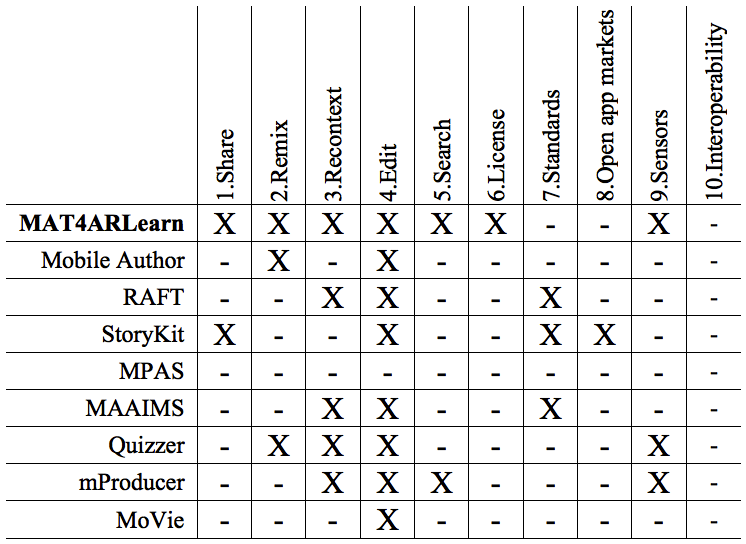
\includegraphics[width=0.9\linewidth]{img/table3}
	\caption{Mobile authoring tools classification according to features.}
	\label{table3} 
\end{figure}



\end{small}



\clearpage{\pagestyle{empty}\cleardoublepage}
%-------------------------------------------------------------------- END

%-------------------------------------------------------------------- START
\begin{Large}
\textbf{Appendix B} 
\end{Large}
\vspace{3em}

\textbf{Here is the title for appendix B}

\begin{small}

AQUI SE METE LA MOVIDA

\end{small}



\clearpage{\pagestyle{empty}\cleardoublepage}
%-------------------------------------------------------------------- END